\section{Debugging your crumb structure}%
\label{section:debugging-crumb-structure}

The crumb structure of your bread provides insights into how well
your fermentation process has gone. You can also spot common flaws
arising from improper technique. This chapter will provide you with information
that you can use to debug your baking process.

\begin{figure}
  \includegraphics[width=\textwidth]{crumb-structures-book}
  \caption{A schematic visualization of different crumb structures and their respective causes. The
  final bread's crumb is a key aspect to identify potential issues related to fermentation
  or baking technique.}%
  \label{fig:crumb-structures-book}
\end{figure}

\subsection{Perfect fermentation}

\begin{figure}
  \includegraphics[width=\textwidth]{open-crumb}
  \caption{The bread has a somewhat open crumb with areas
  featuring a honeycomb structure.}%
  \label{fig:open-crumb}
\end{figure}

Of course the perfect fermentation is debatable and highly subjective. To
me the perfect sourdough bread features a crisp crust paired with a fluffy,
somewhat open crumb. This is the perfect balance of different consistencies
when you take a bite.

Some people are chasers of a very open crumb, meaning you have large pockets
of air (alveoli). It's subjective whether that's the style of bread that you like;
however, to achieve it you need to ferment your bread dough perfectly.
It takes a lot of skill both in terms of mastering fermentation and technique
to achieve a crumb structure like that.

Personally, I~like a bread like that, just with a slightly less wild crumb.
The style of crumb I~like is called the \emph{honeycomb crumb}. It's not too open, but
just enough open to make the bread very fluffy. To achieve the previously mentioned open crumb, you
have to touch your dough as little as possible. The more you interact with your
dough, the more you are degassing your dough. Excess touching of the dough
results in the dough's alveoli merging together. The crumb will not be as open.
That's why achieving such a crumb works best if you only ferment
one loaf at a time. Normally, if you have to pre-shape your dough,
you will automatically degas your dough a little bit during the rounding process.
If you skip this step and directly shape your dough, you will achieve a more open crumb.
A good rule of thumb is to not touch your dough for at least 1--2~hours before shaping,
to achieve as open a crumb as possible.

\begin{figure}
  \includegraphics[width=\textwidth]{honeycomb}
  \caption{A whole wheat sourdough with an almost exclusive honeycomb crumb
  structure.}%
  \label{fig:honeycomb}
\end{figure}


Now this is problematic when you want to
make multiple loaves at the same time. Pre-shaping is essential as you are required
to divide your large bulk dough into smaller chunks. Without the pre-shaping
process, you would end up with many non-uniform bread doughs. This technique is
also used when making ciabattas. They are typically not shaped. You only cut the
bulk dough into smaller pieces, trying to work the dough as little as possible.
With pre-shaping you will converge your dough's alveoli into more of a honeycomb structure,
as large pockets of air will slightly merge. Similarly to the open crumb structure,
you also have to nail the fermentation process perfectly to achieve this crumb.
Too long a fermentation will result in gas leaking out of your dough while baking.
The honeycombs won't be able to retain the gas. If you ferment for too short a time,
there is not enough gas to inflate the structures. To me this is the perfect
style of crumb. As someone who appreciates jam, no jam will fall through a slice
of this bread compared to an open crumb.

\subsection{Overfermented}%
\label{sec:overfermented-dough}

\begin{figure}
  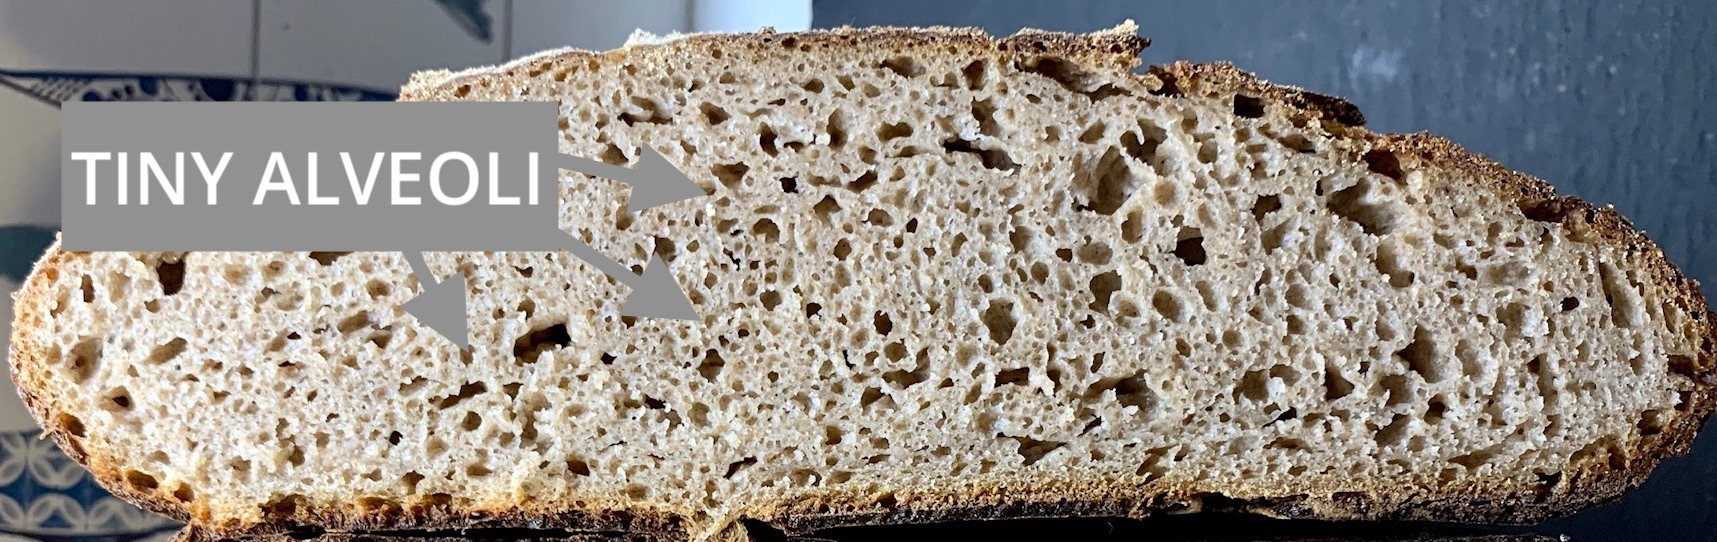
\includegraphics[width=\textwidth]{fermented-too-long}
  \caption{A relatively flat dough that has many tiny pockets of air.}%
  \label{fig:fermented-too-long}
\end{figure}

When fermenting your dough for too long, the protease enzyme starts to
break down the gluten of your flour. Furthermore, the bacteria consume the gluten
in a process called \emph{proteolysis}~\cite{raffaella+di+cagno}.
Bakers also refer to this process as \emph{gluten rot}.
The gluten that normally traps the \ch{CO2} created
by the fermentation process of your microorganisms can no longer keep the
gas inside of the dough. The gas disperses outward resulting in smaller alveoli in your crumb.
The bread itself tends to be very flat in the oven. Bakers often refer
to this style of bread as a \emph{pancake}. The oven spring can be compared
to bread doughs made out of low-gluten flour like einkorn.

Your bread will feature a lot of acidity, a really strong distinctive tang. From
a taste perspective, it might be a little bit too sour. From my own tests with family and
friends (n=15--20), I~can say that this style of bread is typically
appreciated less. However, I~personally really like the hearty strong taste.
It is excellent in combination with something
sweet or a soup.  From a consistency perspective, it is no longer as fluffy as it could be.
The crumb might also taste a little bit gummy. That's because it has been broken down a lot
by the bacteria. Furthermore, this style of bread has a significantly lower amount of gluten~\cite{raffaella+di+cagno}
and is no longer comparable to raw flour, it's a fully fermented product.
You can compare it with a blue cheese that is almost lactose free.

When trying to work with the dough, you will notice that suddenly the dough feels
very sticky. You can no longer properly shape and work the dough. When trying to
remove the dough from a banneton, the dough flattens out a lot. Furthermore,
in many cases your dough might stick to the banneton. When beginning with baking
I~would use a lot of rice flour in my banneton to dry out the surface of the dough a lot.
This way the dough wouldn't stick, despite being overfermented. However as it
turns out the stickiness issue has been my lack of understanding the fermentation
process. Now I~never use rice flour, except when trying to apply decorative scorings.
Properly managing fermentation results in a dough that is not sticky.

If you are noticing, during a stretch and fold or during shaping, that your dough
is suddenly overly sticky, then the best option is to use a loaf pan. Simply take
your dough and toss it into a loaf pan. Wait until the dough mixture has increased
in size a bit again and then bake it. You will have a very good-tasting sourdough
bread. If it's a bit too sour, you can just bake your dough for a longer period
of time to boil away some of the acidity during the baking process. You can also use
your dough to set up a new starter and try again tomorrow. Lastly, if you are hungry,
you can simply pour some of your dough directly into a heated pan with a bit of
oil. It will make delicious sourdough flatbreads.

To fix issues related to over-fermentation, you need to stop the fermentation process
earlier. What I~like to do is to extract a small fermentation sample from my dough.
Depending on the volume increase of this sample, I~can mostly judge when my fermentation
is finished. Try to start with a \qty{25}{\percent} volume increase of your
main dough or sample.  Depending on how much gluten your flour has, you can
ferment for a longer period of time.  With a strong flour featuring a
\qtyrange{14}{15}{\percent} protein, you should be able to safely ferment
until a \qty{100}{\percent} size increase. This however also depends on your
sourdough starter's composition of yeast and bacteria. The more bacterial fermentation,
the faster your dough structure breaks down. Frequent feedings of your sourdough
starter will improve the yeast activity. Furthermore, a stiff sourdough starter
might be a good solution too. The enhanced yeast activity will result in a more fluffy
dough with less bacterial activity. A better yeast activity also will result
in less acidity in your final bread. If you are a chaser of a very strong tangy
flavor profile, then a stronger flour with more gluten will help.


\subsection{Underfermented}

\begin{figure}
  \includegraphics[width=\textwidth]{fermented-too-short-underbaked}
  \caption{A dense dough featuring a gummy, not fully gelatinized area.
  The picture has been provided by the user wahlfeld from our community
Discord server.}%
  \label{fig:fermented-too-short-underbaked}
\end{figure}

This defect is also commonly referred to as \emph{underproofed}. However underproofed
is not a good term as it only refers to having a short final
proofing stage of the bread-making process.
If you were to bake your bread after a perfectly-timed bulk fermentation stage,
the result will not be underproofed even if you skipped the proofing stage entirely.
Proofing will make your dough a bit more extensible and allows your sourdough
to inflate the dough a bit more. When faced with an underfermented bread, something
went wrong earlier during the bulk fermentation stage, or maybe even
before with your sourdough starter.

A typical underfermented dough has very large pockets of air and is partially
wet and gummy in some areas of the dough. The large pockets can be compared
to making a non-leavened wheat or corn tortilla. As you bake the dough in your pan,
the water slowly starts to evaporate. The gas is trapped in the structure of the dough
and will create pockets. In case of a tortilla, this is the desired behavior.
But when you observe this process in a larger dough, you will create several
super alveoli. The water evaporates, and the first alveoli form. Then at some point,
the starch starts to gelatinize and becomes solid. This happens first inside of the pockets
as the interior heats up faster compared to the rest of the dough. Once all the starch
has gelatinized, the alveoli holds their shape and no longer expand. During this
process other parts of the bread dough are pushed outwards. That's why an underfermented
dough sometimes even features an ear during the baking process. This
is also commonly referred to as a \emph{fool's crumb}. You are excited about an ear which
can be quite hard to achieve. Plus you might think you finally created some big pockets
of air in your crumb. But in reality you fermented for too short a period
of time.

\begin{figure}
  \includegraphics[width=\textwidth]{fools-crumb}
  \caption{A typical example of a fool's crumb featuring an ear and several overly
  large alveoli. The picture has been provided by Rochelle from our
  community Discord server.}%
  \label{fools-crumb}
\end{figure}

In a properly fermented dough, the alveoli help with the heat transfer throughout the dough.
From within the many tiny fermentation-induced pockets, the starch gelatinizes. With
an underfermented dough, this heat transfer does not properly work. Because of that
you sometimes have areas which look like raw dough. Bakers refer to this as a very
gummy structure sometimes. Baking your dough for a longer period of time would also properly
gelatinize the starch in these areas. However, then other parts of your bread
might be baked too long.

To fix issues related to under-fermentation, you simply have to ferment your dough
for a longer period of time. Now, there is an upper limit to fermentation time
as your flour starts to break down the moment it is in contact with water. That's why it
might be a good idea to simply speed up your fermentation process. As a rough
figure, I~try to aim for a bulk fermentation time of around 8--12~hours typically.
To achieve that you can try to make your sourdough starter more active.  This can be done
by feeding your starter daily over several days. Use the same ratio as you would
do for your main bread dough. Assuming you use \qty{20}{\percent} starter
calculated on the flour, use a 1:5:5 ratio to feed your starter. That would be
\qty{10}{\gram} of existing starter, \qty{50}{\gram} of flour, \qty{50}{\gram}
of water for instance.  To boost your yeast activity even more, you can
consider making a stiff sourdough 
starter. The bacteria produces mostly acid. The more acidity
is piled up, the less active your yeast is. The stiff sourdough starter
enables you to start your dough's fermentation with stronger yeast activity
and less bacterial activity.

\subsection{Not enough dough strength}

\begin{figure}
  \includegraphics[width=\textwidth]{flat-bread}
  \caption{A very flat bread without enough dough strength.}%
  \label{flat-bread}
\end{figure}

When a dough flattens out quite a lot during the baking process, the chances are
that you did not create enough dough strength. This means your gluten matrix
hasn't been developed properly. Your dough is too extensible and flattens out
mostly rather than springing upwards in the oven. This can also happen if you
proofed your dough for too long. Over time the gluten relaxes and your dough
becomes more and more extensible. You can observe the gluten relaxing behavior
too when making a pizza pie. Directly after shaping your dough balls, it's
very hard to shape the pizza pie. If you wait for 30--90~minutes stretching
the dough becomes a lot easier.

The easiest way to fix this is probably to knead your dough more at the start. To simplify
things consider using less water for your flour too. This will result in a more elastic dough
right away. This concept is commonly used for no-knead style sourdough.  Alternatively, you
can also perform more stretch and folds during the bulk fermentation process. Each
stretch and fold will help to strengthen the gluten matrix and make a more elastic dough.
The last option to fix a dough with too little dough strength is to shape your dough tighter.

\subsection{Baked too hot}

\begin{figure}
  \includegraphics[width=\textwidth]{baked-too-hot-v2}
  \caption{A bread with very large alveoli close to the crust.}%
  \label{baked-too-hot}
\end{figure}

This is a common mistake that has happened to me a lot. When you bake your dough
at too high a temperature, you constrain your dough's expansion. The starch gelatinizes
and becomes more and more solid. At around 140°C (284°F) the Maillard reaction
starts to completely thicken your bread dough's crust. This is similar to baking
your bread dough without steam. As the internal dough's temperature heats up,
more and more water evaporates, gas expands and the dough is being pushed upwards.
Once the dough reaches the crust, it can no longer expand. The alveoli merge
into larger structures close to the surface of the dough. By baking too hot,
you are not achieving the ear which adds extra flavor. Furthermore, by restricting
it's expansion, the crumb will not be as fluffy as it could be.

If you have an extensible dough with high hydration, baking too cold will result
in the dough flattening out quite a lot. The gelatinization of the starch is
essential for the dough to hold its structure. After conducting several
experiments, it seems that my sweet spot for maximum oven spring seems to be
at around 230°C (446°F). Test the temperature of your oven, because in several
cases the displayed temperature might not match the actual temperature of your
oven~\cite{too+hot+baking}. Make sure to turn off the fan of your oven. Most
home ovens are designed to vent the steam as fast as possible. If you can not
turn the fan off, consider using a Dutch oven.

\subsection{Baked with too little steam}

\begin{figure}[h]
  \includegraphics[width=\textwidth]{no-steam}
  \caption{One of my earlier breads that I~baked at a friend's place where
  I~couldn't steam the dough properly.}%
  \label{no-steam}
\end{figure}

Similar to baking too hot, when baking without enough steam, your dough's crust
forms too quickly. It's hard to spot the difference between the two mistakes.
I~typically first ask about the temperature and then about the steaming technique
to determine what might be wrong with the baking process. Too little steam can
typically be spotted by having a thick crust around all around your dough paired
with large alveoli towards the edges.

The steam essentially prevents the Maillard reaction from happening too quickly
on your crust. That's why steaming during the first stages of the bake is so important.
The steam keeps the temperature of your crust close to around 100°C (212°F). Achieving steam
can be done by using a Dutch oven, an inverted tray and/or a bowl of boiling water.
You might also have an oven with a built-in steam functionality. All the methods work,
it depends on what you have at hand. My default go-to method is an inverted
tray on top of my dough, paired with a bowl full of boiling water towards the bottom
of the oven.

\begin{figure}[ht]
  \includegraphics[width=\textwidth]{apple-experiment-temperatures}
  \caption{An apple with 2 probes to measure ambient
  and surface temperatures of several steaming techniques
  in a Dutch oven.}%
  \label{apple-experiment-temperatures}
\end{figure}

Now there can also be too much steam. For this I~tested using a Dutch oven paired with large ice
cubes to provide additional steam. The temperature of my dough's surface would directly
jump close to 100°C. The steam contains more energy and thus through convection
can heat up the surface of your dough faster. I~tested this by putting an apple inside
a Dutch oven and measuring its surface temperature using a barbecue thermometer.
I~then changed the steaming methods to plot how quickly the temperature
close to the surface changes. I~tested an ice cube inside of a preheated
Dutch oven, a preheated Dutch oven, a preheated Dutch oven with spritzes
of water on the apple's surface, a non-preheated Dutch oven where I~would only preheat
the bottom part. The experiment then showed that the ice-cube method would heat up
the surface of the apple a lot quicker. When replicating this with a bread dough,
I~would achieve less oven spring.

\begin{figure}[ht]
  \includegraphics[width=\textwidth]{apple-experiment-surface-temperatures}
  \caption{A chart showing how the temperature of the surface
  of the apple changes with different steaming techniques.}%
  \label{apple-experiment-surface-temperatures}
\end{figure}

\begin{figure}[ht]
  \includegraphics[width=\textwidth]{apple-experiment-ambient-temperatures}
  \caption{This figure shows how the ambient temperatures inside of the
  Dutch oven change depending on the steaming technique that is used.}%
  \label{apple-experiment-ambient-temperatures}
\end{figure}

Generally though, achieving too much steam is relatively challenging. I~could only
make this mistake when using a Dutch oven as the steaming method paired with relatively
large ice cubes. After talking with other bakers using the same Dutch oven, it seems
that my ice cubes (around \qty{80}{\gram}) were 4 times as heavy as the ones
other bakers would use (\qty{20}{\gram}).
